\documentclass[12pt]{article}
\usepackage[top=1in,left=1in, right = 1in, footskip=1in]{geometry}

\usepackage{graphicx}
\usepackage{xspace}
%\usepackage{adjustbox}

\newcommand{\comment}{\showcomment}
%% \newcommand{\comment}{\nocomment}

\newcommand{\showcomment}[3]{\textcolor{#1}{\textbf{[#2: }\textsl{#3}\textbf{]}}}
\newcommand{\nocomment}[3]{}

\newcommand{\jd}[1]{\comment{cyan}{JD}{#1}}
\newcommand{\swp}[1]{\comment{magenta}{SWP}{#1}}
\newcommand{\bmb}[1]{\comment{blue}{BMB}{#1}}
\newcommand{\djde}[1]{\comment{red}{DJDE}{#1}}

\newcommand{\eref}[1]{Eq.~\ref{eq:#1}}
\newcommand{\fref}[1]{Fig.~\ref{fig:#1}}
\newcommand{\Fref}[1]{Fig.~\ref{fig:#1}}
\newcommand{\sref}[1]{Sec.~\ref{#1}}
\newcommand{\frange}[2]{Fig.~\ref{fig:#1}--\ref{fig:#2}}
\newcommand{\tref}[1]{Table~\ref{tab:#1}}
\newcommand{\tlab}[1]{\label{tab:#1}}
\newcommand{\seminar}{SE\mbox{$^m$}I\mbox{$^n$}R}

\usepackage{amsthm}
\usepackage{amsmath}
\usepackage{amssymb}
\usepackage{amsfonts}

\usepackage{lineno}
\linenumbers

\usepackage[pdfencoding=auto, psdextra]{hyperref}

\usepackage{natbib}
\bibliographystyle{chicago}
\date{\today}

\usepackage{xspace}
\newcommand*{\ie}{i.e.\@\xspace}

\usepackage{color}

\newcommand{\Rx}[1]{\ensuremath{{\mathcal R}_{#1}}\xspace} 
\newcommand{\Ro}{\Rx{0}}
\newcommand{\Rc}{\Rx{\mathrm{c}}}
\newcommand{\RR}{\ensuremath{{\mathcal R}}\xspace}
\newcommand{\Rhat}{\ensuremath{{\hat\RR}}}
\newcommand{\Rnaive}{\ensuremath{{\mathcal R}_{\textrm{\tiny naive}}}\xspace}
\newcommand{\tsub}[2]{#1_{{\textrm{\tiny #2}}}}
\newcommand{\dd}[1]{\ensuremath{\, \mathrm{d}#1}}
\newcommand{\dtau}{\dd{\tau}}
\newcommand{\dx}{\dd{x}}
\newcommand{\dsigma}{\dd{\sigma}}

\newcommand{\tstart}{\ensuremath{\tsub{t}{start}}\xspace}
\newcommand{\tend}{\ensuremath{\tsub{t}{end}}\xspace}

\newcommand{\betaeff}{\ensuremath{\tsub{\beta}{eff}}\xspace}
\newcommand{\Keff}{\ensuremath{\tsub{K}{eff}}\xspace}

\newcommand{\pt}{p} %% primary time
\newcommand{\st}{s} %% secondary time

\newcommand{\psize}{{\mathcal P}} %% primary cohort size
\newcommand{\ssize}{{\mathcal S}} %% secondary cohort size

\newcommand{\gtime}{\sigma} %% generation interval
\newcommand{\gdist}{g} %% generation-interval distribution

\newcommand{\geff}{g_{\textrm{eff}}} %% generation-interval distribution

\newcommand{\total}{{\mathcal T}} %% total number of serial intervals

\newcommand{\PP}{{\mathcal P}}
\newcommand{\II}{{\mathcal I}}

\begin{document}

\begin{flushleft}{
	\Large
	\textbf\newline{
		Quantifying the effects of population- and individual-based intervention strategies
	}
}
\newline
\\
Sang Woo Park\textsuperscript{1,*}
\\
\bigskip
\textbf{1} Department of Ecology and Evolutionary Biology, Princeton University, Princeton, NJ, USA
\\
\bigskip

*Corresponding author: swp2@princeton.edu
\end{flushleft}


\section{Introduction}

\section{Methods}

\subsection{Renewal equation framework}

We begin by describing the uncontrolled spread of infection using the renewal equation framework.
Let $K(\tau)$ represent the intrinsic infection kernel, defined as the rate at which infectious contacts are made by an average infected individual infected $\tau$ time units ago in the absence of any intervention.
The integral of $K(\tau)$, representing the total infectiousness of an average infected individual, corresponds to the basic reproduction number: $\Ro = \int K(\tau) \dtau$.
The kernel, normalized by the total infectiousness, corresponds to the intrinsic generation-interval distribution: $g(\tau) = K(\tau)/\Ro$.
While the generation interval is typically defined as the time between when an individual is infected and when that individual infects another person, it is more convenient to think of the intrinsic generation-interval distribution as time distribution of infectious \emph{contacts} (which will result in infection if the contactee is susceptible).
Then, the rate at which an individual infected $\tau$ time units ago will generate a secondary case at calendar time $t$---the effective kernel, $\Keff(t,\tau)$---can be written as a product between the proportion susceptible in $S$ and infection kernel $K$:
\begin{equation}
\Keff(t,\tau) = S(t) K(\tau).
\end{equation}
Likewise, we can also define the forward kernel $F_t(\tau)$ which describes the rate at which an individual infected at time $t$ will generate a secondary case $\tau$ time units after infection:
\begin{equation}
F_t(\tau) = S(t+\tau) K(\tau) = \Keff(t+\tau,\tau).
\end{equation}
While both effective and forward kernels provide valid measures for describing temporal variation in infectiousness, one can be more useful than the other depending on the purpose.
The forward kernel is particularly convenient because it capture how infectiousness varies over the course of an individual's infection and therefore is directly related to realized generation intervals (i.e., time between actual infection events);
in particular, the (forward) realized generation-interval distribution $f_t(\tau)$ can be obtained by normalizing the forward kernel:
\begin{equation}
f_t(\tau) = \frac{F_t(\tau)}{\int_0^\infty F_t(\tau) \dtau}.
\end{equation}
Ignoring births and deaths, we can further express the dynamics of the proportion susceptible $S(t)$ and incidence $i(t)$ in the absence of intervention as follows:
\begin{align}
\frac{\mathrm{d}S}{\mathrm{d}t} &= - i(t),\\
i(t) &= \int_0^\infty F_{t-\tau}(\tau) i(t-\tau) \dtau,\\
&=\int_0^\infty \Keff(t,\tau) i(t-\tau) \dtau,\\
&= S(t) \int_0^\infty K(\tau) i(t-\tau) \dtau.
\end{align}
This model, also known as renewal equations, generalizes the dynamics of many compartmental models.

\subsection{Population- and individual-based intervention}

\begin{figure}[!th]
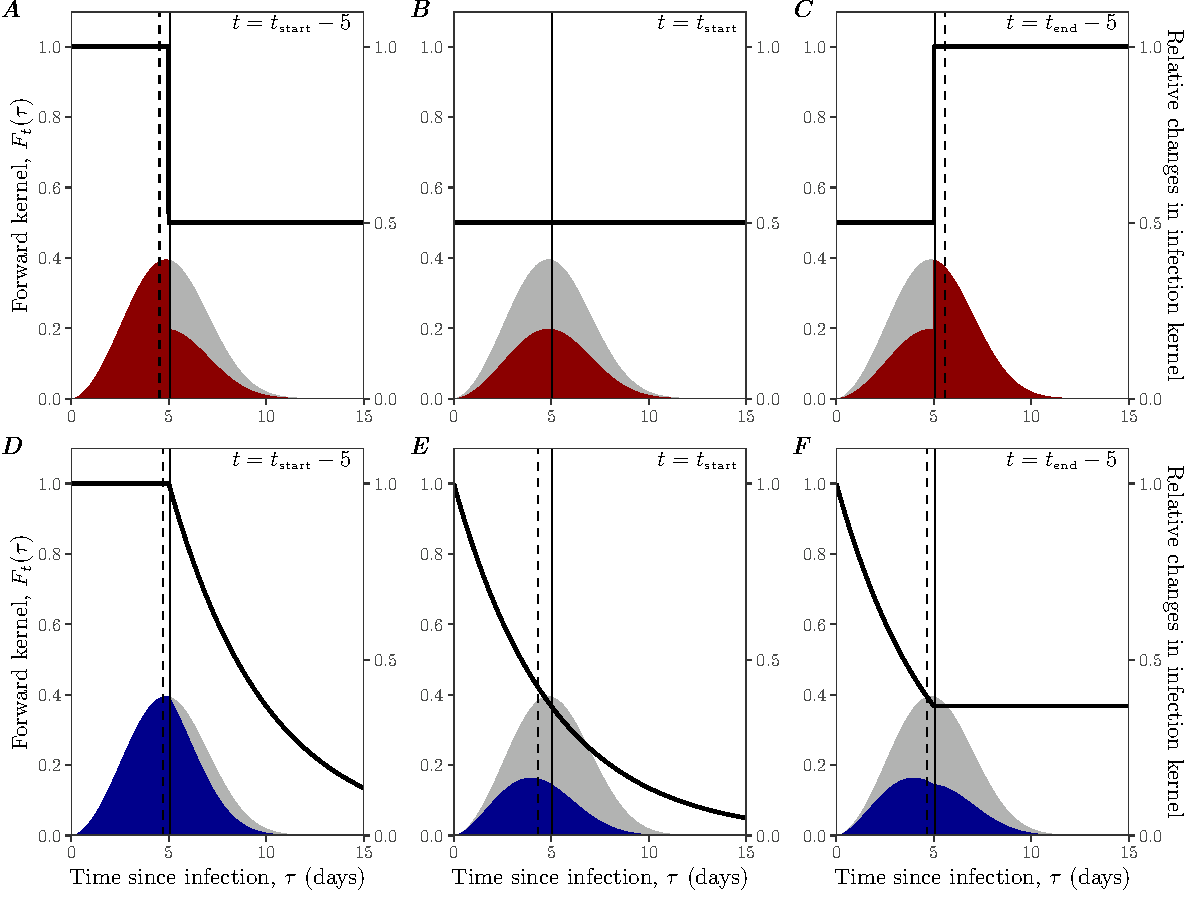
\includegraphics[width=1\textwidth]{pop_ind_compare.pdf}
\caption{
\textbf{I'm a caption}
}
\label{fig:indpop}
\end{figure}

To model the impact of intervention during an ongoing epidemic, we first distinguish population-based interventions, which equally affect the transmission potential of all infected individuals regardless of their time of infection, from individual-based interventions, which target each individual and therefore depend on the time of infection.
Population-based interventions can be thought of as interventions that reduce the transmission rate and include social distancing, school closures, and vaccination.
Individual-based interventions can be thought of as interventions that reduce the duration of infectious periods and include case identification and isolation.
Some interventions, like contact tracing, are conceptually analogous to individual-based interventions but are mathematically different from population- and individual-based interventions because they depend not only on the infection time of an infected individual but also on their infector's infection time;
for simplicity, we do not consider these at this stage.

Let $\PP(t)$ represent a population-based intervention that modulates the infection kernel multiplicatively at calendar time $t$ such that $\PP(t)=1$ corresponds to intervention that has no effect and $\PP(t) < 1$ corresponds to intervention that reduces transmission.
Then, the effective kernel under $\PP$ at calendar time $t$ can be written as:
\begin{equation}
\Keff(t, \tau) = S(t) \PP(t) K(\tau).
\end{equation}
Likewise, the forward kernel of an individual infected at time $t$ under $\PP$ can be written as:
\begin{equation}
F_t(\tau) = S(t+\tau) \PP(t + \tau) K(\tau).
\end{equation}
Here, we see that population-based intervention has same impact on transmission dynamics as susceptible depletion.
This intervention is also strength-like because \swp{...}.
Since we assume that population-based intervention affects infection kernel multiplicatively, it is straightforward to model multiple interventions occurring throughout an epidemic: $\PP(t) = \prod_{i=1}^n \PP_i(t)$.

For example, a social distancing measure that reduces transmission potential by a factor of $1/\phi$ between time \tstart and \tend can be modeled as:
\begin{equation}
\PP(t) = \begin{cases}
1 & t < \tstart\\
\phi & \tstart \leq t < \tend\\
1 & \tend \leq t
\end{cases}.
\end{equation}
\fref{indpop}A--C illustrates the impact of such intervention on the forward kernel of an individual infected 5 days before $\tstart$, at $\tstart$, and 5 days before $\tend$ (assuming $S(t) \approx 1$).
Population-based interventions can take effect immediately and sharply reduce transmission (\fref{indpop}A);
likewise, lifting the intervention can, in theory, cause the forward kernel to return back to normal immediately (\fref{indpop}C).
Even though the exact shape of the kernel depends on the time of infection and when the intervention was introduced relative to the infection time, the relative impact of intervention in reducing transmission at any given time (by a factor of $1/\phi$) does not vary across individuals (\fref{indpop}A--C).
Such intervention also has direct effects on realized generation intervals:
implementing (lifting) intervention decreases (increases) future transmission potential and therefore decreases (increases) the mean realized generation interval (\fref{indpop}A,C).
If an individual is infected after \tstart (and much earlier than \tend), this intervention simply reduces the entire kernel by a constant amount and has no effect on realized generation intervals.
This mechanism explains and further generalizes how susceptible depletion leads to contraction of generation intervals in a homogeneously mixing population. 

On the other hand, individual-based intervention $\II(t, \tau)$, such as case isolation, targets each infected individual and therefore depends on calendar time $t$ as well as time since infection $\tau$.
In particular, we interpret $\II(t,\tau)$ as the probability that an individual infected $\tau$ time units ago has not been isolated by calendar time $t$ such that $\II(t, \tau) < 1$ represents reduction in transmission.
In this case, the effective kernel under $\II$ at calendar time $t$ is given by:
\begin{equation}
\Keff(t, \tau) = S(t) \II(t, \tau) K(\tau).
\end{equation}
Likewise, the forward kernel of an individual infected at time $t$ under $\II$ can be written as:
\begin{equation}
F_t(\tau) = S(t+\tau) \II(t+\tau, \tau) K(\tau).
\end{equation}
This intervention is speed-like because its effectiveness depends on how fast we can isolate infected individuals.

For example, given hazard $h(\tau)$ of being isolated, the probability that an individual infected at time $t$ has not been isolated by $\tau$ time units after infection given that the individual-based intervention takes place between time \tstart and \tend depends on the amount of time the individual has been exposed to this intervention.
If the individual was infected before $\tstart$, they will not be isolated until after $\tstart$.
If the individual was infected after $\tend$, they will never be isolated.
Therefore, such probability can be modeled as:
\begin{equation}
\II(t+\tau, \tau) = \begin{cases}
1 & t < \tstart-\tau \\
\exp\left(- \int_{\max(0, \tstart - t)}^{\min(\tau, \tend-t)} h(s)\dd{s} \right) & \tstart-\tau \leq t < \tend \\
1 & \tend \leq t
\end{cases}
\end{equation}
Like population-based intervention, multiple individual-based interventions can be modeled using competing hazards ($h(\tau)=\sum_{i=1}^m h_i(\tau)$), which in turn can be expressed as product of interventions: $\II(t,\tau) = \prod_{i=1}^n \II_i(t,\tau)$.
\fref{indpop}D--E illustrates the impact of a single individual-based intervention with constant hazard on the forward kernel of an individual infected 5 days before $\tstart$, at $\tstart$, and 5 days before $\tend$ (assuming $S(t) \approx 1$).
Unlike the population-based intervention, individual-based intervention does not take effect immediately;
that is, the rate at which an infected individual generates a secondary case at time $\tstart$ (e.g., $F_t(\tstart-t)$ in \fref{indpop}D; more generally, $K(\tstart, \tau)$) remains unaffected by the intervention because it takes time to identify and isolate infected individuals.
On the other hand, when the intervention is lifted at $\tend$, the value of the kernel at calendar time $\tend$ ($F_t(\tend-t)$ in \fref{indpop}F; more generally, $K(\tend, \tau)$) remains unchanged because some fraction of infected individuals have already been isolated.
In general, individual-based interventions shorten realized generation intervals because they prevent late transmission (\fref{indpop}D--E).

Finally, given (possibly multiple) population- and individual-based interventions, $P(t)$ and $I(t, \tau)$, the effective kernel can be written as:
\begin{equation}
\Keff(t, \tau) = S(t) \PP(t) \II(t,\tau) K(\tau).
\end{equation}
The corresponding forward kernel can be written as:
\begin{equation}
F_t(\tau) = S(t+\tau) \PP(t + \tau) \II(t+\tau, \tau) K(\tau).
\end{equation}
Therefore, the dynamics of $S(t)$ and $i(t)$ can be now written as:
\begin{equation}
\begin{aligned}
\frac{\mathrm{d}S}{\mathrm{d}t} &= - i(t),\\
i(t) &= \int_0^\infty F_{t-\tau}(\tau) i(t-\tau) \dtau,\\
&=\int_0^\infty  \Keff(t,\tau) i(t-\tau)\dtau,\\
&= S(t) \PP(t) \int_0^\infty \II(t, \tau) K(\tau) i(t-\tau)\dtau.
\label{eq:renewal}
\end{aligned}
\end{equation}

\subsection{Quantifying changes in time-dependent reproduction number}

The impact of intervention is often measured by the instantaneous reproduction number $\RR(t)$, which is defined as the average number of secondary cases caused by a primary case infected at time $t$ given conditions at time $t$:
\begin{align}
\RR(t) &= \int_0^\infty \Keff(t, \tau) \dtau,\\
&= \RR_0 S(t) \PP(t) \int_0^\infty \II(t,\tau) g(\tau) \dtau.
\label{eq:rt}
\end{align}
Since $\RR(t)$ measures conditions at time $t$, we expect to observe changes in $\RR(t)$ as soon as intervention is implemented.

In order to estimate $\RR(t)$, we first define the effective generation-interval by normalizing the effective kernel:
\begin{align}
\geff(t, \tau) &= \frac{\Keff(t, \tau)}{\RR(t)},\\
&= \frac{\II(t,\tau) g(\tau)}{\int_0^\infty \II(t,\tau') g(\tau') \dtau'}.
\label{eq:geff}
\end{align}
Then, by substituting \eref{rt} into \eref{renewal} and rearranging, we can show that:
\begin{equation}
\begin{aligned}
\frac{\mathrm{d}S}{\mathrm{d}t} &= - i(t),\\
i(t) &= \RR(t) \int_0^\infty \geff(t, \tau) i(t-\tau) \dtau.
\end{aligned}
\end{equation}
This yields a novel estimator for $\RR(t)$:
\begin{equation}
\RR(t) = \frac{i(t)}{\int_0^\infty \geff(t, \tau) i(t-\tau) \dtau}.
\end{equation}
While this estimator is similar in form to previously proposed estimators, the main difference is that it allows for the underlying generation-interval distribution to vary to account for individual-based intervention (\eref{geff}).
In particular, Cori et al have popularized the estimation of $\RR(t)$ via the R package EpiEstim, but it also assumes that the underlying generation-interval distribution does not change over time; 
such method accurately captures changes in $\RR(t)$ under population-based intervention, but not under individual-based intervention.

In general, when both population- and individual-based interventions are present during an ongoing epidemic, the classical estimator that assumes a time-invariant generation-interval distribution measures a slightly different quantity.
Given incidence between time $0$ and $t-\epsilon$ for $\epsilon > 0$, we can calculate the proportional reduction $p(t)$ in true incidence $i(t)$ at time $t$ compared to incidence that we would observe in the absence of intervention:
\begin{align}
p(t) &= \frac{S(t) \PP(t) \int_0^\infty \II(t, \tau) K(\tau) i(t-\tau)\dtau}{S(t) \int_0^\infty K(\tau) i(t-\tau) \dtau}\\
\end{align}
By substituting true incidence $i(t)$ in the numerator and rearranging, we obtain the classical expression for the estimator for $\RR(t)$---which we refer to as $\tsub{\RR}{prop}(t)$---that depends on the proportion of the susceptible population and proportional reduction in incidence, rather than proportional reduction in transmission:
\begin{equation}
\tsub{\RR}{prop}(t) = \Ro S(t) p(t) = \frac{i(t)}{\int_0^\infty i(t-\tau) g(\tau) \dtau}.
\end{equation}

\subsection{Quantifying changes in the effective generation-interval distribution}

In order to accurately estimate the instantaneous reproduction number, we have to be able to first quantify how the effective generation-interval distribution $\geff(t, \tau)$ changes across time $t$.
The effective distribution measures the infectiousness of an individual infected $\tau$ time units ago at time $t$ and therefore is different from the distribution of realized generation intervals (i.e., time between actual infection events).
For example, if we were to take all realized generation intervals that end at time $t$ and form a distribution, we obtain what is known as the backward generation-interval distribution, $b_t(\tau)$:
\begin{align}
b_t(\tau) &= \frac{i(t-\tau) \Keff(t,\tau)}{\int_0^\infty i(t-x) \Keff(t,x) \dx},\\
&= \frac{i(t-\tau) \geff(t,\tau)}{\int_0^\infty i(t-x) \geff(t,x) \dx},
\end{align}
which is, in fact, a convolution of the effective generation-interval distribution with previous incidence of infection.

Some studies have suggested substituting the forward distribution $f_t(\tau)$, including the forward serial-interval distribution, instead to estimate $\RR(t)$:
\begin{equation}
\tsub{\RR}{forward}(t) = \frac{i(t)}{\int_0^\infty i(t-\tau) f_{t-\tau}(\tau) \dtau}.
\end{equation}
However, this choice is also suboptimal.
While both the forward generation-interval distribution $f_{t-\tau}(\tau)$ and the effective generation-interval distribution $g(t)(\tau)$ depend on the number of secondary cases at time $t$ caused by a primary case infected at time $t-\tau$, $K(t, \tau)$, they are normalized by different quantities:
\begin{equation}
f_{t-\tau}(\tau) = \frac{K(t,\tau)}{\int_0^\infty K(t-\tau+x,x) \dx} \neq \frac{K(t,\tau)}{\int_0^\infty K(t,x) \dx} = \geff(t, \tau).
\end{equation}
The forward distribution $f_{t-\tau}(\tau)$ is normalized by the average number of secondary cases caused by a primary case infected at time $t-\tau$.
On the other hand, the effective distribution $\geff(t, \tau)$ is normalized by the sum of average number of secondary cases that an individual infected at time $t-x$ will generate at time $t$ (integrated across $x$).

Therefore, even if we can observe all realized generation intervals throughout an epidemic, estimating the effective distribution $\geff(t, \tau)$ is not trivial.
Either a deconvolution or a novel statistical tool is needed to estimate the effective distribution $\geff(\tau)$.
To our knowledge, no studies have accomplished this yet.

\subsection{Example: Semi-mechanistic SIR model}

In order to understand how population- and individual-based interventions affect disease spread, we use a semi-mechanistic SIR model to generate synthetic data and compare estimates of $\RR(t)$:
\begin{align}
\frac{\dd{S}}{\dd{t}} &= - \beta(t)S I,\\
\frac{\dd{I}}{\dd{t}} &= \beta(t)S I - \gamma(t) I,\\
\frac{\dd{R}}{\dd{t}} &= \gamma(t) I,
\end{align}
where $S$, $I$, $R$ represent proportion of individuals that are susceptible, infected, and removed;
$\beta(t)$ represent time-varying transmission rate; and $\gamma(t)$ represent time-varying removal rate.
This model is semi-mechanistic because it allows $\beta$ and $\gamma$ to change over time but their changes are not necessarily driven by any particular mechanism.
In this case, the effective kernel can be written as:
\begin{equation}
K(t, \tau) = \beta(t) S(t) \exp\left(-\int_{t-\tau}^t \gamma(s) \dd{s} \right).
\end{equation}
Here, we see that changes in transmission rate $\beta(t)$ and removal rate $\gamma(t)$ correspond to population- and individual-based intervention.
In particular, abrupt changes in $\gamma(t)$ does not affect the incidence at time $t^\ast$ due to delays in isolating individuals.
Finally, the instantaneous reproduction number is given by:
\begin{equation}
\RR(t) = \beta(t) S(t) \int_0^\infty \exp\left(-\int_{t-\tau}^t \gamma(s) \dd{s} \right) \dtau.
\end{equation}
When $\gamma(t) = \gamma(0)$, we obtain a familiar form: $\RR(t) = \Ro S(t)$,
where $\Ro = \beta(0)/\gamma(0)$.

Here, we consider a simple scenario in which a flu-like pathogen $\Ro = 1.5$ invades an immunologically naive population.
In the beginning, the disease spreads without any intervention.
On day 25, an intense case isolation measure is implemented. 
On day 40, the intervention is completely/partially lifted.
This is modeled as follows:
\begin{equation}
\beta(t) = 3/10\,\,\textrm{days}^{-1}, \gamma(t) = \begin{cases}
1/5\,\, \textrm{days}^{-1} & t < 25\\
1/2\,\, \textrm{days}^{-1} & 25 \leq t < 40 \\
\tsub{\gamma}{late} & 40 \leq t
\end{cases},
\end{equation}
where we vary $\tsub{\gamma}{late}$ between $1/3\,\, \textrm{days}^{-1}$ and $1/5\,\, \textrm{days}^{-1}$
Initial conditions are specified as follows: $S(0) = 1 - 10^{-3}$, $I(0) = 10^{-3}$, and $R(0) = 0$.
We run the simulation for 100 days and compute instantaneous incidence $i(t) = \beta(t) S I$. 
Then, we compare $\RR(t)$ with $\tsub{\RR}{prop}(t)$.

Since we assume that incidence is known exactly, we can, in fact, estimate the transmission rate $\beta(t)$ (with fixed $\gamma(t)=\gamma(0)$) that gives identical incidence trajectory until time $t$.
This transmission rate is given by:
\begin{equation}
\beta(t) = \frac{\tsub{\RR}{prop}(t)\gamma(0)}{S(t)}.
\end{equation}



\end{document}
